\section{Termodinamikaning ikkinchi qonuni. Issiqlik mashinalari}



\begin{enumerate}

\item Issiqlik mashinasining ishchi jismi bo‘lgan gaz ichki energiyasining bir sikl davomidagi o‘zgarishini toping. Sikl davomida gaz isitkichdan $Q_1$ issiqlik miqdori oladi, sovitkichga $Q_2$ issiqlik miqdori beradi va $A$ ish bajaradi.
\begin{enumerate}[label=\Alph*)]
\item $Q_1 - Q_2 + A$
\item $Q_1 - Q_2$
\item $A - Q_1 - Q_2$
\item 0
\end{enumerate}

\item Real issiqlik mashinasi FIK ifodasini ko‘rsating.
\begin{enumerate}[label=\Alph*)]
\item $\frac{Q_1 - Q_2}{Q_2} \cdot 100\%$
\item $\frac{Q_1 - Q_2}{Q_1} \cdot 100\%$
\item $\frac{Q_2 - Q_1}{Q_1} \cdot 100\%$
\item $\frac{T_1 - T_2}{T_1} \cdot 100\%$
\end{enumerate}

\item Real issiqlik mashinasida ishchi qism isitkichdan 2 kJ issiqlik olib, sovitkichga 600 J issiqlik berdi. Uning bajargan foydali ishini toping (J).
\begin{enumerate}[label=\Alph*)]
\item 2600
\item 2000
\item 1400
\item 600
\end{enumerate}

\item Real issiqlik mashinasida ishchi qism isitkichdan 600 J issiqlik olib, 400 J foydali ish bajardi. U sovitkichga qancha issiqlik bergan (J)?
\begin{enumerate}[label=\Alph*)]
\item 1000
\item 2000
\item 0
\item 600
\end{enumerate}

\item Real issiqlik mashinasi 520 J foydali ish bajardi. Bunda sovitkichga 180 J issiqlik berildi. Ishchi qism isitkichdan qancha issiqlik olgan (J)?
\begin{enumerate}[label=\Alph*)]
\item 700
\item 0
\item 180
\item 520
\end{enumerate}

\item Issiqlik mashinasi sikl davomida isitkichdan 100 J issiqlik oldi va sovitkichga 60 J issiqlik berdi. Mashinaning FIK ni toping.
\begin{enumerate}[label=\Alph*)]
\item 67\%
\item 60\%
\item 40\%
\item 25\%
\end{enumerate}

\item FIK $\eta$ bo‘lgan issiqlik mashinasi isitkichdan $Q$ issiqlik miqdori olganda qanday ish bajaradi?
\begin{enumerate}[label=\Alph*)]
\item $\eta Q$
\item $(1 + \eta)Q$
\item $(1 - \eta)Q$
\item $Q / \eta$
\end{enumerate}

\item Issiqlik dvigateli isitkichdan har sekundda 7200 kJ issiqlik oladi va sovitkichga 6400 kJ issiqlik beradi. Dvigatelning FIK qanday?
\begin{enumerate}[label=\Alph*)]
\item 62\%
\item 41\%
\item 24\%
\item 11\%
\end{enumerate}

\item Issiqlik dvigateli isitkichdan 0,8 MJ issiqlik miqdori olib, sovitkichga 0,3 MJ issiqlik miqdorini beradi. Bu issiqlik dvigatelining FIK ni (\%) toping.
\begin{enumerate}[label=\Alph*)]
\item 30
\item 48
\item 50
\item 62,5
\end{enumerate}

\item Issiqlik dvigateli isitkichdan 0,4 MJ issiqlik miqdori olib, sovitkichga 0,26 MJ issiqlik miqdorini uzatadi. Dvigatelning FIK ni hisoblang (\%).
\begin{enumerate}[label=\Alph*)]
\item 30
\item 35
\item 40
\item 45
\end{enumerate}

\item Bitta siklda issiqlik mashinasi 28 kJ ish bajarib, sovitkichga 42 kJ issiqlik miqdorini beradi. Mashinaning FIK ni aniqlang (\%).
\begin{enumerate}[label=\Alph*)]
\item 30
\item 42
\item 40
\item 50
\end{enumerate}

\item FIK 25\% bo‘lgan issiqlik mashinasi sovitkichga 600 J issiqlik beradi. U qanday foydali ish bajaradi (J)?
\begin{enumerate}[label=\Alph*)]
\item 200
\item 300
\item 400
\item 500
\end{enumerate}

\item FIK 40\% bo‘lgan issiqlik mashinasi bitta siklda sovitkichga 42 kJ issiqlik beradi. Mashina bitta siklda necha kJ ish bajaradi?
\begin{enumerate}[label=\Alph*)]
\item 21
\item 28
\item 168
\item 56
\end{enumerate}

\item Issiqlik mashinasining FIK 25\%. Uning isitkichdan olgan issiqlik miqdori 800 J bo‘lsa, foydali ishi necha Joul bo‘ladi?
\begin{enumerate}[label=\Alph*)]
\item 100
\item 200
\item 300
\item 400
\end{enumerate}

\item Foydali ish koeffitsienti 30\% bo‘lgan ideal issiqlik mashinasi qizdirgichdan 10 kJ issiqlik oladi. Sovitkichga berilayotgan issiqlik miqdori qanday (kJ)?
\begin{enumerate}[label=\Alph*)]
\item 6
\item 7
\item 3
\item 2,4
\end{enumerate}

\item Isitkichning harorati $150^\circ C$, sovitkichniki $20^\circ C$. Ideal issiqlik mashinasining FIK necha foiz?
\begin{enumerate}[label=\Alph*)]
\item 20
\item 23
\item 25
\item 30,7
\end{enumerate}

\item Ideal issiqlik mashina isitkichining harorati $117^\circ C$, sovitkichniki $27^\circ C$. Mashinaning FIK ni toping (\%).
\begin{enumerate}[label=\Alph*)]
\item 23
\item 33
\item 70
\item 30
\end{enumerate}

\item Karno siklida ishlayotgan issiqlik mashinasiga temperaturasi $480^\circ C$ bo‘lgan bug‘ kirib, undan $30^\circ C$ temperaturada chiqsa, mashinaning FIK qanday (\%)?
\begin{enumerate}[label=\Alph*)]
\item 30
\item 40
\item 50
\item 60
\end{enumerate}

\item Bug‘ turbinasiga bug‘ $500^\circ C$ harorat bilan kirib, undan $30^\circ C$ harorat bilan chiqib ketadi. Bug‘ turbinasini ideal issiqlik mashinasi deb hisoblab, uning FIK ni toping (\%).
\begin{enumerate}[label=\Alph*)]
\item 30
\item 47
\item 61
\item 77
\end{enumerate}

\item Isitkichining harorati $227^\circ C$, sovitkichniki $27^\circ C$ bo‘lgan issiqlik mashinasining maksimal FIK necha foiz?
\begin{enumerate}[label=\Alph*)]
\item 20
\item 30
\item 40
\item 45
\end{enumerate}

\item FIK ning maksimal qiymati 50\% bo‘lishi uchun isitkichining harorati $527^\circ C$ bo‘lgan issiqlik mashinasi sovitkichining harorati qanday ($^\circ C$) bo‘lishi kerak?
\begin{enumerate}[label=\Alph*)]
\item 400
\item 351
\item 263,5
\item 127
\end{enumerate}

\item Isitkichining harorati 500 K bo‘lgan issiqlik mashinasining FIK 50\%. Sovitkichning harorati qanday (K)?
\begin{enumerate}[label=\Alph*)]
\item 190
\item 200
\item 230
\item 250
\end{enumerate}

\item FIK ning maksimal qiymati 70\% bo‘lishi uchun isitkichining harorati $727^\circ C$ bo‘lgan issiqlik mashinasi sovitkichining harorati qanday ($^\circ C$) bo‘lishi kerak?
\begin{enumerate}[label=\Alph*)]
\item 27
\item 218
\item 300
\item 315
\end{enumerate}

\item Isitkich harorati $427^\circ C$ bo‘lib, sovitkich harorati $127^\circ C$. Issiqlik mashinasi bir siklda 600 J issiqlik olib, sovitkichga 400 J issiqlik beradi. Real mashinaning FIK ideal mashina FIK ning qancha qismini tashkil qiladi?
\begin{enumerate}[label=\Alph*)]
\item 1/2
\item 6/7
\item 7/8
\item 7/9
\end{enumerate}

\item FIK $\eta$ bo‘lgan issiqlik dvigatelida gaz bajargan ishni 13 marta oshirish uchun isitkichdan olinadigan issiqlik miqdorini qanday o‘zgartirish kerak? $\eta = const$.
\begin{enumerate}[label=\Alph*)]
\item $13/\eta$ marta orttirish
\item 13 marta orttirish
\item 13 marta kamaytirish
\item $13\eta$ marta orttirish
\end{enumerate}

\item Karno siklida ishlaydigan mashinada isitkich va sovitkich absolyut temperaturalarining nisbati 5 ga teng. Agar bir siklda sovitkichga 36 kJ issiqlik berilgan bo‘lsa, isitkichdan olingan issiqlik miqdori qanday (kJ)?
\begin{enumerate}[label=\Alph*)]
\item 900
\item 180
\item 72
\item 7,2
\end{enumerate}

\item Ideal issiqlik mashinasi bir sikl davomida $5,36 \cdot 10^4$ J ish bajardi. Isitkich temperaturasi $100^\circ C$, sovitkichniki esa $0^\circ C$ bo‘lsa, mashina bir siklda isitkichdan qanday (kJ) issiqlik miqdori oladi?
\begin{enumerate}[label=\Alph*)]
\item 150
\item 170
\item 200
\item 210
\end{enumerate}

\item Isitkichining temperaturasi $T_1$, sovitkichining temperaturasi $T_2$ bo‘lgan issiqlik mashinasi bor. $T_1$ ni $\Delta T$ ga orttirib, $T_2$ ni o‘zgartirmagan va $T_2$ ni $\Delta T$ ga kamaytirib, $T_1$ ni o‘zgartirmagan hollardagi FIK larning nisbatini toping.
\begin{enumerate}[label=\Alph*)]
\item $\frac{T_1 - \Delta T}{T_1}$
\item $\frac{T_1 + \Delta T}{T_2 + \Delta T}$
\item $\frac{T_1}{T_1 + \Delta T}$
\item $\frac{T_1 - T_2}{T_1}$
\end{enumerate}

\item Rasmda ko‘rsatilgan siklning qaysi qismida gaz manfiy ish bajaradi?

\begin{tikzpicture}[>=stealth, scale=1]
    % Koordinata o'qlari
    \draw[->, thick] (0,0) -- (4,0) node[right] {$T$};
    \draw[->, thick] (0,0) -- (0,3.5) node[above] {$P$};
    \node[below left] at (0,0) {$O$};

    % Nuqtalarni belgilash
    \coordinate (1) at (1.5, 1.2);
    \coordinate (2) at (1.5, 2.5);
    \coordinate (3) at (3, 2.5);

    % 1-2 jarayon (Izotermik siqilish - T=const, P ortmoqda)
    \draw[thick, ->] (1) -- (2);
    \node[left] at (1) {1};
    \node[left] at (2) {2};

    % 2-3 jarayon (Izobarik kengayish - P=const, T ortmoqda)
    \draw[thick, ->] (2) -- (3);
    \node[above] at (3) {3};

    % 3-1 jarayon (Izoxorik sovish - V=const, chiziq koordinata boshiga yo'nalgan)
    \draw[thick, ->] (3) -- (1);
    \draw[dashed] (0,0) -- (1);

\end{tikzpicture}

\begin{enumerate}[label=\Alph*)]
\item bunda gaz manfiy ish bajarmaydi
\item 2-3
\item 1-2
\item 3-1
\end{enumerate}

\item Gazning rasmda ko‘rsatilgan siklni o‘tishda bajargan ishini toping.

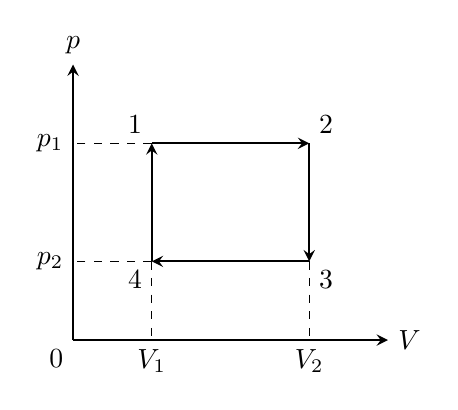
\begin{tikzpicture}[>=stealth, scale=1]
    % Koordinata o'qlari
    \draw[->, thick] (0,0) -- (4,0) node[right] {$V$};
    \draw[->, thick] (0,0) -- (0,3.5) node[above] {$p$};
    \node[below left] at (0,0) {0};

    % Nuqtalar koordinatalari
    \coordinate (1) at (1, 2.5);
    \coordinate (2) at (3, 2.5);
    \coordinate (3) at (3, 1);
    \coordinate (4) at (1, 1);

    % Sikl chizig'i va yo'nalish strelkalari
    \draw[thick, ->] (1) -- (2);
    \draw[thick, ->] (2) -- (3);
    \draw[thick, ->] (3) -- (4);
    \draw[thick, ->] (4) -- (1);

    % Nuqta raqamlari
    \node[above left] at (1) {1};
    \node[above right] at (2) {2};
    \node[below right] at (3) {3};
    \node[below left] at (4) {4};

    % O'qlardagi proyeksiyalar va labellar
    \draw[dashed] (1) -- (0, 2.5) node[left] {$p_1$};
    \draw[dashed] (4) -- (0, 1) node[left] {$p_2$};
    \draw[dashed] (4) -- (1, 0) node[below] {$V_1$};
    \draw[dashed] (3) -- (3, 0) node[below] {$V_2$};
\end{tikzpicture}

\begin{enumerate}[label=\Alph*)]
\item $(p_1 - p_2)(V_2 - V_1)$
\item $p_2(V_2 - V_1)$
\item $(p_1 - p_2)V_1$
\item $(p_1 - p_2)V_2$
\end{enumerate}

\item Rasmda ko‘rsatilgan siklda bajarilgan ishni quyidagi ifodalarning qaysi biridan foydalanib topish mumkin?

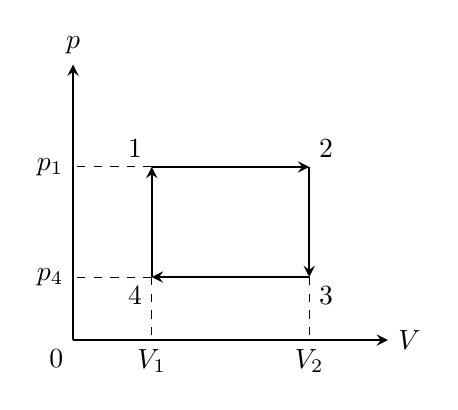
\begin{tikzpicture}[>=stealth, scale=1]
    % Koordinata o'qlari
    \draw[->, thick] (0,0) -- (4,0) node[right] {$V$};
    \draw[->, thick] (0,0) -- (0,3.5) node[above] {$p$};
    \node[below left] at (0,0) {0};

    % Nuqtalar koordinatalari
    \coordinate (A) at (1, 2.2);
    \coordinate (B) at (3, 2.2);
    \coordinate (C) at (3, 0.8);
    \coordinate (D) at (1, 0.8);

    % Sikl chizig'i va yo'nalish strelkalari
    \draw[thick, ->] (A) -- (B);
    \draw[thick, ->] (B) -- (C);
    \draw[thick, ->] (C) -- (D);
    \draw[thick, ->] (D) -- (A);

    % Nuqta raqamlari
    \node[above left] at (A) {1};
    \node[above right] at (B) {2};
    \node[below right] at (C) {3};
    \node[below left] at (D) {4};

    % O'qlardagi proyeksiyalar (formula uchun zaruriy parametrlar)
    \draw[dashed] (A) -- (0, 2.2) node[left] {$p_1$};
    \draw[dashed] (D) -- (0, 0.8) node[left] {$p_4$};
    \draw[dashed] (D) -- (1, 0) node[below] {$V_1$};
    \draw[dashed] (C) -- (3, 0) node[below] {$V_2$};
\end{tikzpicture}

\begin{enumerate}[label=\Alph*)]
\item $(p_1 + p_2)(V_2 - V_1)$
\item $p_2(V_2 - V_1)$
\item $(p_1 - p_4)(V_2 - V_1)$
\item $p_1(V_2 - V_1)$
\end{enumerate}

\item Diagrammada ko‘rsatilgan sikl bo‘yicha ishlovchi issiqlik mashinasi bir sikl davomida qanday (kJ) ish bajaradi?

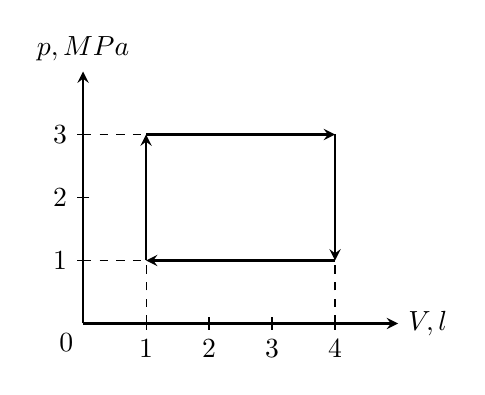
\begin{tikzpicture}[>=stealth, scale=0.8]
    % Koordinata o'qlari
    \draw[->, thick] (0,0) -- (5,0) node[right] {$V, l$};
    \draw[->, thick] (0,0) -- (0,4) node[above] {$p, \text{MPa}$};
    \node[below left] at (0,0) {0};

    % O'qlardagi bo'linmalar (V o'qi)
    \foreach \x in {1,2,3,4}
        \draw (\x, 0.1) -- (\x, -0.1) node[below] {\x};
        
    % O'qlardagi bo'linmalar (p o'qi)
    \foreach \y in {1,2,3}
        \draw (0.1, \y) -- (-0.1, \y) node[left] {\y};

    % Sikl nuqtalari
    \coordinate (A) at (1,1);
    \coordinate (B) at (1,3);
    \coordinate (C) at (4,3);
    \coordinate (D) at (4,1);

    % Sikl chiziqlari va yo'nalish strelkalari (Clockwise)
    \draw[thick, ->] (A) -- (B); % Izoxorik isitish
    \draw[thick, ->] (B) -- (C); % Izobarik kengayish
    \draw[thick, ->] (C) -- (D); % Izoxorik sovutish
    \draw[thick, ->] (D) -- (A); % Izobarik siqilish

    % Proyeksiya chiziqlari (punktir)
    \draw[dashed] (1,0) -- (1,1);
    \draw[dashed] (4,0) -- (4,1);
    \draw[dashed] (0,1) -- (1,1);
    \draw[dashed] (0,3) -- (1,3);

\end{tikzpicture}

\begin{enumerate}[label=\Alph*)]
\item 3
\item 6
\item 8
\item 9
\end{enumerate}

\item Diagrammada ko‘rsatilgan sikl bo‘yicha ishlovchi issiqlik mashinasi bir sikl davomida qanday (kJ) ish bajaradi?

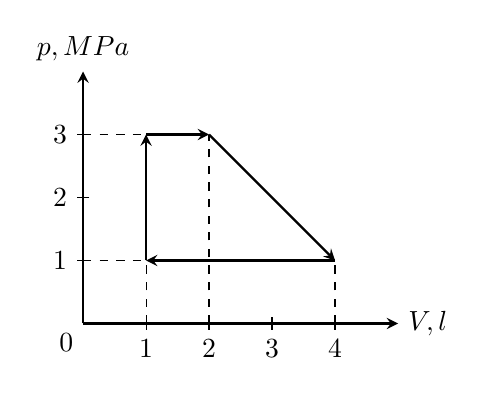
\begin{tikzpicture}[>=stealth, scale=0.8]
    % Koordinata o'qlari
    \draw[->, thick] (0,0) -- (5,0) node[right] {$V, l$};
    \draw[->, thick] (0,0) -- (0,4) node[above] {$p, \text{MPa}$};
    \node[below left] at (0,0) {0};

    % V o'qidagi bo'linmalar
    \foreach \x in {1,2,3,4}
        \draw (\x, 0.1) -- (\x, -0.1) node[below] {\x};
        
    % p o'qidagi bo'linmalar
    \foreach \y in {1,2,3}
        \draw (0.1, \y) -- (-0.1, \y) node[left] {\y};

    % Sikl nuqtalari koordinatalari
    \coordinate (A) at (1,1);
    \coordinate (B) at (1,3);
    \coordinate (C) at (2,3);
    \coordinate (D) at (4,1);

    % Sikl chiziqlari va yo'nalish strelkalari
    \draw[thick, ->] (A) -- (B); % Izoxorik isitish (1 -> 3 MPa)
    \draw[thick, ->] (B) -- (C); % Izobarik kengayish (1 -> 2 l)
    \draw[thick, ->] (C) -- (D); % O'zgaruvchan jarayon (diagonall)
    \draw[thick, ->] (D) -- (A); % Izobarik siqilish (4 -> 1 l)

    % Proyeksiya (punktir) chiziqlari
    \draw[dashed] (1,0) -- (1,1);
    \draw[dashed] (2,0) -- (2,3);
    \draw[dashed] (4,0) -- (4,1);
    \draw[dashed] (0,1) -- (1,1);
    \draw[dashed] (0,3) -- (1,3);

\end{tikzpicture}

\begin{enumerate}[label=\Alph*)]
\item 3
\item 4
\item 6
\item 7
\end{enumerate}

\end{enumerate}



\begin{table}[h!]
\centering
\begin{tabular}{|c|c|c|c|c|c|c|c|c|c|}
\hline
№ & J. & № & J. & № & J. & № & J. & № & J. \\ \hline
1 & D & 8 & D & 15 & B & 22 & D & 29 & C \\ \hline
2 & B & 9 & D & 16 & D & 23 & A & 30 & A \\ \hline
3 & C & 10 & B & 17 & A & 24 & D & 31 & C \\ \hline
4 & B & 11 & C & 18 & D & 25 & B & 32 & B \\ \hline
5 & A & 12 & A & 19 & C & 26 & B & 33 & B \\ \hline
6 & C & 13 & B & 20 & C & 27 & C & & \\ \hline
7 & A & 14 & B & 21 & D & 28 & C & & \\ \hline
\end{tabular}
\end{table}